\PassOptionsToPackage{unicode=true}{hyperref} % options for packages loaded elsewhere
\PassOptionsToPackage{hyphens}{url}
\PassOptionsToPackage{dvipsnames,svgnames*,x11names*}{xcolor}
%
\documentclass[ngerman,a4paper,]{scrartcl}
\usepackage{lmodern}
\usepackage{amssymb,amsmath}
\usepackage{ifxetex,ifluatex}
\usepackage{fixltx2e} % provides \textsubscript
\ifnum 0\ifxetex 1\fi\ifluatex 1\fi=0 % if pdftex
  \usepackage[T1]{fontenc}
  \usepackage[utf8]{inputenc}
  \usepackage{textcomp} % provides euro and other symbols
\else % if luatex or xelatex
  \usepackage{unicode-math}
  \defaultfontfeatures{Ligatures=TeX,Scale=MatchLowercase}
    \setmainfont[]{Source Serif Pro}
    \setsansfont[]{Source Sans Pro}
    \setmonofont[Mapping=tex-ansi,Mapping=tex-ansi,Scale=0.8]{Source Code Pro}
  \setmathfont[]{Asana Math}
\fi
% use upquote if available, for straight quotes in verbatim environments
\IfFileExists{upquote.sty}{\usepackage{upquote}}{}
% use microtype if available
\IfFileExists{microtype.sty}{%
\usepackage[]{microtype}
\UseMicrotypeSet[protrusion]{basicmath} % disable protrusion for tt fonts
}{}
\IfFileExists{parskip.sty}{%
\usepackage{parskip}
}{% else
\setlength{\parindent}{0pt}
\setlength{\parskip}{6pt plus 2pt minus 1pt}
}
\usepackage{xcolor}
\usepackage{hyperref}
\hypersetup{
            pdftitle={Bookdown Deployment Experiments},
            pdfauthor={Lukas Burk},
            colorlinks=true,
            linkcolor=Maroon,
            citecolor=Blue,
            urlcolor=Blue,
            breaklinks=true}
\urlstyle{same}  % don't use monospace font for urls
\usepackage{color}
\usepackage{fancyvrb}
\newcommand{\VerbBar}{|}
\newcommand{\VERB}{\Verb[commandchars=\\\{\}]}
\DefineVerbatimEnvironment{Highlighting}{Verbatim}{commandchars=\\\{\}}
% Add ',fontsize=\small' for more characters per line
\usepackage{framed}
\definecolor{shadecolor}{RGB}{248,248,248}
\newenvironment{Shaded}{\begin{snugshade}}{\end{snugshade}}
\newcommand{\AlertTok}[1]{\textcolor[rgb]{0.94,0.16,0.16}{#1}}
\newcommand{\AnnotationTok}[1]{\textcolor[rgb]{0.56,0.35,0.01}{\textbf{\textit{#1}}}}
\newcommand{\AttributeTok}[1]{\textcolor[rgb]{0.77,0.63,0.00}{#1}}
\newcommand{\BaseNTok}[1]{\textcolor[rgb]{0.00,0.00,0.81}{#1}}
\newcommand{\BuiltInTok}[1]{#1}
\newcommand{\CharTok}[1]{\textcolor[rgb]{0.31,0.60,0.02}{#1}}
\newcommand{\CommentTok}[1]{\textcolor[rgb]{0.56,0.35,0.01}{\textit{#1}}}
\newcommand{\CommentVarTok}[1]{\textcolor[rgb]{0.56,0.35,0.01}{\textbf{\textit{#1}}}}
\newcommand{\ConstantTok}[1]{\textcolor[rgb]{0.00,0.00,0.00}{#1}}
\newcommand{\ControlFlowTok}[1]{\textcolor[rgb]{0.13,0.29,0.53}{\textbf{#1}}}
\newcommand{\DataTypeTok}[1]{\textcolor[rgb]{0.13,0.29,0.53}{#1}}
\newcommand{\DecValTok}[1]{\textcolor[rgb]{0.00,0.00,0.81}{#1}}
\newcommand{\DocumentationTok}[1]{\textcolor[rgb]{0.56,0.35,0.01}{\textbf{\textit{#1}}}}
\newcommand{\ErrorTok}[1]{\textcolor[rgb]{0.64,0.00,0.00}{\textbf{#1}}}
\newcommand{\ExtensionTok}[1]{#1}
\newcommand{\FloatTok}[1]{\textcolor[rgb]{0.00,0.00,0.81}{#1}}
\newcommand{\FunctionTok}[1]{\textcolor[rgb]{0.00,0.00,0.00}{#1}}
\newcommand{\ImportTok}[1]{#1}
\newcommand{\InformationTok}[1]{\textcolor[rgb]{0.56,0.35,0.01}{\textbf{\textit{#1}}}}
\newcommand{\KeywordTok}[1]{\textcolor[rgb]{0.13,0.29,0.53}{\textbf{#1}}}
\newcommand{\NormalTok}[1]{#1}
\newcommand{\OperatorTok}[1]{\textcolor[rgb]{0.81,0.36,0.00}{\textbf{#1}}}
\newcommand{\OtherTok}[1]{\textcolor[rgb]{0.56,0.35,0.01}{#1}}
\newcommand{\PreprocessorTok}[1]{\textcolor[rgb]{0.56,0.35,0.01}{\textit{#1}}}
\newcommand{\RegionMarkerTok}[1]{#1}
\newcommand{\SpecialCharTok}[1]{\textcolor[rgb]{0.00,0.00,0.00}{#1}}
\newcommand{\SpecialStringTok}[1]{\textcolor[rgb]{0.31,0.60,0.02}{#1}}
\newcommand{\StringTok}[1]{\textcolor[rgb]{0.31,0.60,0.02}{#1}}
\newcommand{\VariableTok}[1]{\textcolor[rgb]{0.00,0.00,0.00}{#1}}
\newcommand{\VerbatimStringTok}[1]{\textcolor[rgb]{0.31,0.60,0.02}{#1}}
\newcommand{\WarningTok}[1]{\textcolor[rgb]{0.56,0.35,0.01}{\textbf{\textit{#1}}}}
\usepackage{longtable,booktabs}
% Fix footnotes in tables (requires footnote package)
\IfFileExists{footnote.sty}{\usepackage{footnote}\makesavenoteenv{longtable}}{}
\usepackage{graphicx,grffile}
\makeatletter
\def\maxwidth{\ifdim\Gin@nat@width>\linewidth\linewidth\else\Gin@nat@width\fi}
\def\maxheight{\ifdim\Gin@nat@height>\textheight\textheight\else\Gin@nat@height\fi}
\makeatother
% Scale images if necessary, so that they will not overflow the page
% margins by default, and it is still possible to overwrite the defaults
% using explicit options in \includegraphics[width, height, ...]{}
\setkeys{Gin}{width=\maxwidth,height=\maxheight,keepaspectratio}
% Make links footnotes instead of hotlinks:
\DeclareRobustCommand{\href}[2]{#2\footnote{\url{#1}}}
\setlength{\emergencystretch}{3em}  % prevent overfull lines
\providecommand{\tightlist}{%
  \setlength{\itemsep}{0pt}\setlength{\parskip}{0pt}}
\setcounter{secnumdepth}{5}
% Redefines (sub)paragraphs to behave more like sections
\ifx\paragraph\undefined\else
\let\oldparagraph\paragraph
\renewcommand{\paragraph}[1]{\oldparagraph{#1}\mbox{}}
\fi
\ifx\subparagraph\undefined\else
\let\oldsubparagraph\subparagraph
\renewcommand{\subparagraph}[1]{\oldsubparagraph{#1}\mbox{}}
\fi

% set default figure placement to htbp
\makeatletter
\def\fps@figure{htbp}
\makeatother

\usepackage{booktabs}
\ifnum 0\ifxetex 1\fi\ifluatex 1\fi=0 % if pdftex
  \usepackage[shorthands=off,main=ngerman]{babel}
\else
  % load polyglossia as late as possible as it *could* call bidi if RTL lang (e.g. Hebrew or Arabic)
  \usepackage{polyglossia}
  \setmainlanguage[]{german}
\fi
\usepackage[]{natbib}
\bibliographystyle{apalike}

\title{Bookdown Deployment Experiments}
\author{Lukas Burk}
\date{Stand: 07. May 2020 04:26 Uhr}

\begin{document}
\maketitle

{
\hypersetup{linkcolor=}
\setcounter{tocdepth}{2}
\tableofcontents
}
\hypertarget{prerequisites}{%
\section{Prerequisites}\label{prerequisites}}

This is a \emph{sample} book written in \textbf{Markdown}. You can use anything that Pandoc's Markdown supports, e.g., a math equation \(a^2 + b^2 = c^2\).

The \textbf{bookdown} package can be installed from CRAN or Github:

\begin{Shaded}
\begin{Highlighting}[]
\KeywordTok{install.packages}\NormalTok{(}\StringTok{"bookdown"}\NormalTok{)}
\CommentTok{# or the development version}
\CommentTok{# devtools::install_github("rstudio/bookdown")}
\end{Highlighting}
\end{Shaded}

Remember each Rmd file contains one and only one chapter, and a chapter is defined by the first-level heading \texttt{\#}.

To compile this example to PDF, you need XeLaTeX. You are recommended to install TinyTeX (which includes XeLaTeX): \url{https://yihui.org/tinytex/}.

\hypertarget{intro}{%
\section{Introduction}\label{intro}}

You can label chapter and section titles using \texttt{\{\#label\}} after them, e.g., we can reference Chapter \ref{intro}. If you do not manually label them, there will be automatic labels anyway, e.g., Chapter \ref{methods}.

Figures and tables with captions will be placed in \texttt{figure} and \texttt{table} environments, respectively.

\begin{Shaded}
\begin{Highlighting}[]
\KeywordTok{par}\NormalTok{(}\DataTypeTok{mar =} \KeywordTok{c}\NormalTok{(}\DecValTok{4}\NormalTok{, }\DecValTok{4}\NormalTok{, }\FloatTok{.1}\NormalTok{, }\FloatTok{.1}\NormalTok{))}
\KeywordTok{plot}\NormalTok{(pressure, }\DataTypeTok{type =} \StringTok{'b'}\NormalTok{, }\DataTypeTok{pch =} \DecValTok{19}\NormalTok{)}
\end{Highlighting}
\end{Shaded}

\begin{figure}

{\centering 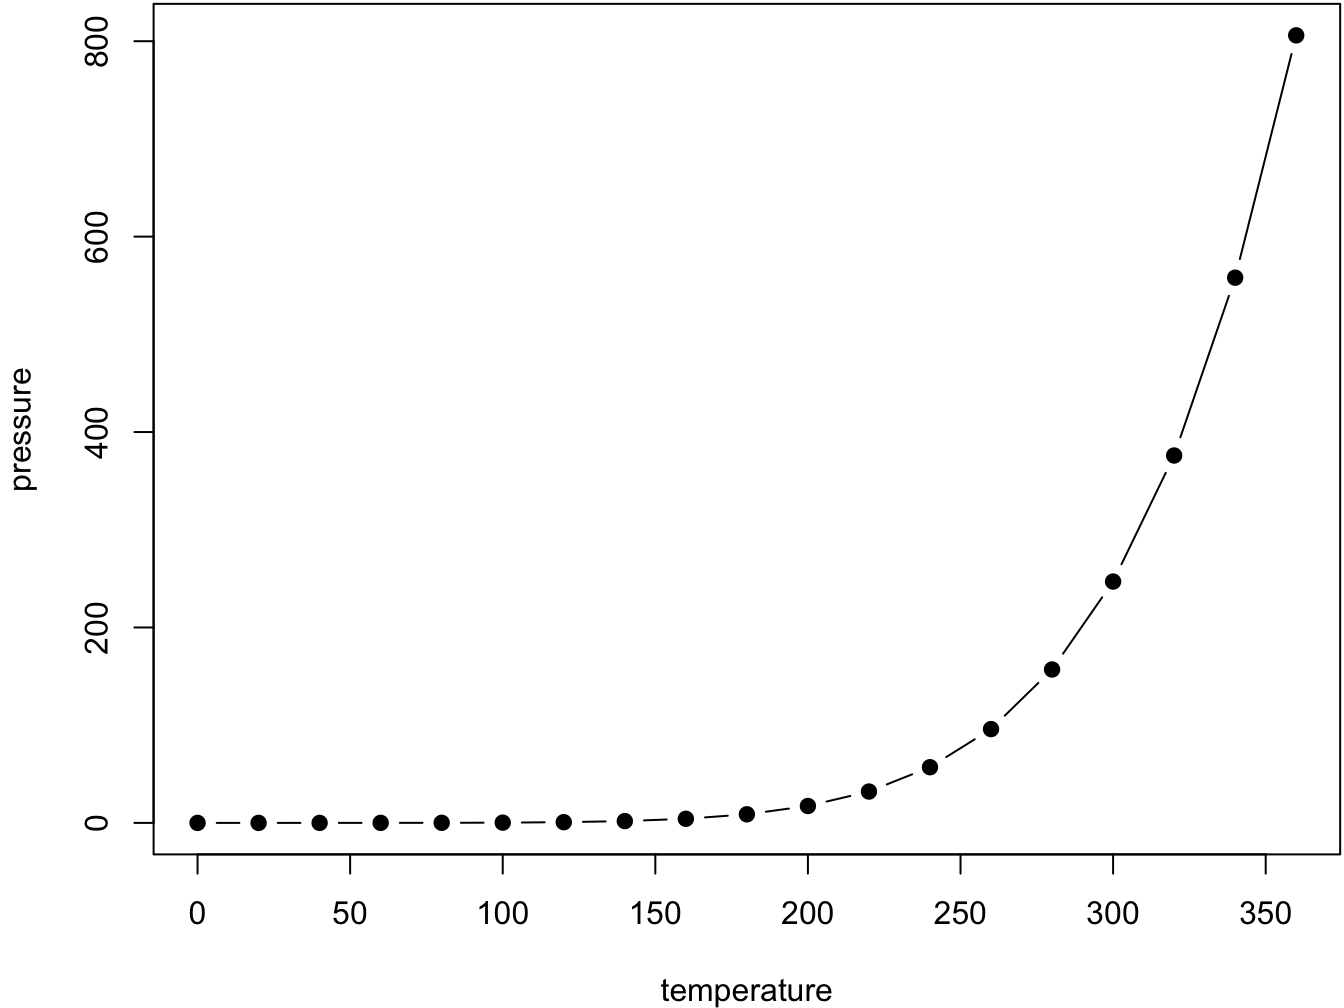
\includegraphics[width=0.8\linewidth]{bookdown-debugging_files/figure-latex/nice-fig-1} 

}

\caption{Here is a nice figure!}\label{fig:nice-fig}
\end{figure}

Reference a figure by its code chunk label with the \texttt{fig:} prefix, e.g., see Figure \ref{fig:nice-fig}. Similarly, you can reference tables generated from \texttt{knitr::kable()}, e.g., see Table \ref{tab:nice-tab}.

\begin{Shaded}
\begin{Highlighting}[]
\NormalTok{knitr}\OperatorTok{::}\KeywordTok{kable}\NormalTok{(}
  \KeywordTok{head}\NormalTok{(iris, }\DecValTok{20}\NormalTok{), }\DataTypeTok{caption =} \StringTok{'Here is a nice table!'}\NormalTok{,}
  \DataTypeTok{booktabs =} \OtherTok{TRUE}
\NormalTok{)}
\end{Highlighting}
\end{Shaded}

\begin{table}

\caption{\label{tab:nice-tab}Here is a nice table!}
\centering
\begin{tabular}[t]{rrrrl}
\toprule
Sepal.Length & Sepal.Width & Petal.Length & Petal.Width & Species\\
\midrule
5.1 & 3.5 & 1.4 & 0.2 & setosa\\
4.9 & 3.0 & 1.4 & 0.2 & setosa\\
4.7 & 3.2 & 1.3 & 0.2 & setosa\\
4.6 & 3.1 & 1.5 & 0.2 & setosa\\
5.0 & 3.6 & 1.4 & 0.2 & setosa\\
\addlinespace
5.4 & 3.9 & 1.7 & 0.4 & setosa\\
4.6 & 3.4 & 1.4 & 0.3 & setosa\\
5.0 & 3.4 & 1.5 & 0.2 & setosa\\
4.4 & 2.9 & 1.4 & 0.2 & setosa\\
4.9 & 3.1 & 1.5 & 0.1 & setosa\\
\addlinespace
5.4 & 3.7 & 1.5 & 0.2 & setosa\\
4.8 & 3.4 & 1.6 & 0.2 & setosa\\
4.8 & 3.0 & 1.4 & 0.1 & setosa\\
4.3 & 3.0 & 1.1 & 0.1 & setosa\\
5.8 & 4.0 & 1.2 & 0.2 & setosa\\
\addlinespace
5.7 & 4.4 & 1.5 & 0.4 & setosa\\
5.4 & 3.9 & 1.3 & 0.4 & setosa\\
5.1 & 3.5 & 1.4 & 0.3 & setosa\\
5.7 & 3.8 & 1.7 & 0.3 & setosa\\
5.1 & 3.8 & 1.5 & 0.3 & setosa\\
\bottomrule
\end{tabular}
\end{table}

You can write citations, too. For example, we are using the \textbf{bookdown} package \citep{R-bookdown} in this sample book, which was built on top of R Markdown and \textbf{knitr} \citep{xie2015}.

\hypertarget{literature}{%
\section{Literature}\label{literature}}

Here is a review of existing methods.

\hypertarget{methods}{%
\section{Methods}\label{methods}}

\hypertarget{plotting}{%
\subsection{Plotting}\label{plotting}}

With FONTS!

\begin{Shaded}
\begin{Highlighting}[]
\KeywordTok{library}\NormalTok{(extrafont) }\CommentTok{# For fontstuff}
\end{Highlighting}
\end{Shaded}

\begin{verbatim}
## Registering fonts with R
\end{verbatim}

\begin{Shaded}
\begin{Highlighting}[]
\CommentTok{# for PDF output}
\KeywordTok{loadfonts}\NormalTok{()}
\KeywordTok{fonttable}\NormalTok{()}
\end{Highlighting}
\end{Shaded}

\begin{verbatim}
## data frame with 0 columns and 0 rows
\end{verbatim}

\begin{Shaded}
\begin{Highlighting}[]
\CommentTok{# using ragg for png}
\CommentTok{# loading just for renv to pick it up}
\KeywordTok{library}\NormalTok{(ragg)}
\end{Highlighting}
\end{Shaded}

\begin{Shaded}
\begin{Highlighting}[]
\KeywordTok{library}\NormalTok{(ggplot2)}

\NormalTok{p <-}\StringTok{ }\KeywordTok{ggplot}\NormalTok{(iris, }\KeywordTok{aes}\NormalTok{(}\DataTypeTok{x =}\NormalTok{ Species, }\DataTypeTok{y =}\NormalTok{ Sepal.Length, }\DataTypeTok{color =}\NormalTok{ Species, }\DataTypeTok{fill =}\NormalTok{ Species)) }\OperatorTok{+}
\StringTok{   }\KeywordTok{geom_boxplot}\NormalTok{(}\DataTypeTok{alpha =} \FloatTok{.75}\NormalTok{, }\DataTypeTok{show.legend =} \OtherTok{FALSE}\NormalTok{) }\OperatorTok{+}
\StringTok{   }\KeywordTok{scale_color_brewer}\NormalTok{(}\DataTypeTok{palette =} \StringTok{"Dark2"}\NormalTok{, }\DataTypeTok{aesthetics =} \KeywordTok{c}\NormalTok{(}\StringTok{"color"}\NormalTok{, }\StringTok{"fill"}\NormalTok{)) }\OperatorTok{+}
\StringTok{   }\KeywordTok{labs}\NormalTok{(}
      \DataTypeTok{title =} \StringTok{"Yet another iris plot"}\NormalTok{,}
      \DataTypeTok{x =} \StringTok{"I should google those species"}\NormalTok{,}
      \DataTypeTok{y =} \StringTok{"*Googleing 'Sepal'*"}\NormalTok{,}
      \DataTypeTok{caption =} \StringTok{"Hi!"}
\NormalTok{   )}

\NormalTok{p }\OperatorTok{+}\StringTok{ }\KeywordTok{theme_minimal}\NormalTok{() }\OperatorTok{+}
\StringTok{   }\KeywordTok{labs}\NormalTok{(}\DataTypeTok{subtitle =} \StringTok{"Whatever this default font is"}\NormalTok{)}
\end{Highlighting}
\end{Shaded}

\begin{figure}
\centering
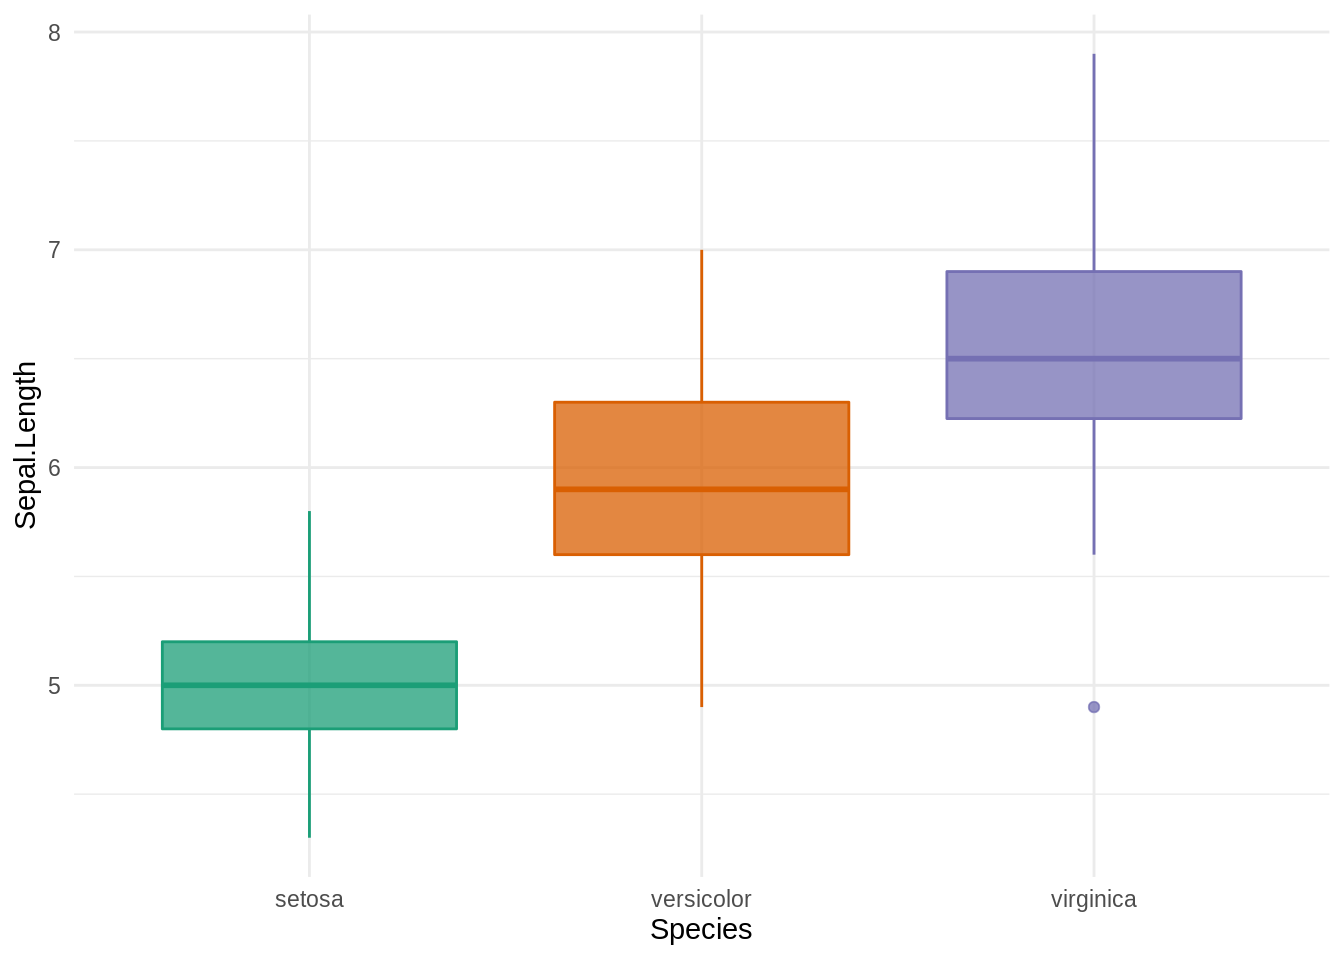
\includegraphics{bookdown-debugging_files/figure-latex/plotting-1-1.pdf}
\caption{\label{fig:plotting-1-1}A plot.}
\end{figure}

\begin{Shaded}
\begin{Highlighting}[]
\NormalTok{p }\OperatorTok{+}\StringTok{ }\KeywordTok{theme_minimal}\NormalTok{(}\DataTypeTok{base_family =} \StringTok{"Source Sans Pro"}\NormalTok{) }\OperatorTok{+}
\StringTok{   }\KeywordTok{labs}\NormalTok{(}\DataTypeTok{subtitle =} \StringTok{"Using Source Sans Pro"}\NormalTok{)}
\end{Highlighting}
\end{Shaded}

\begin{figure}
\centering
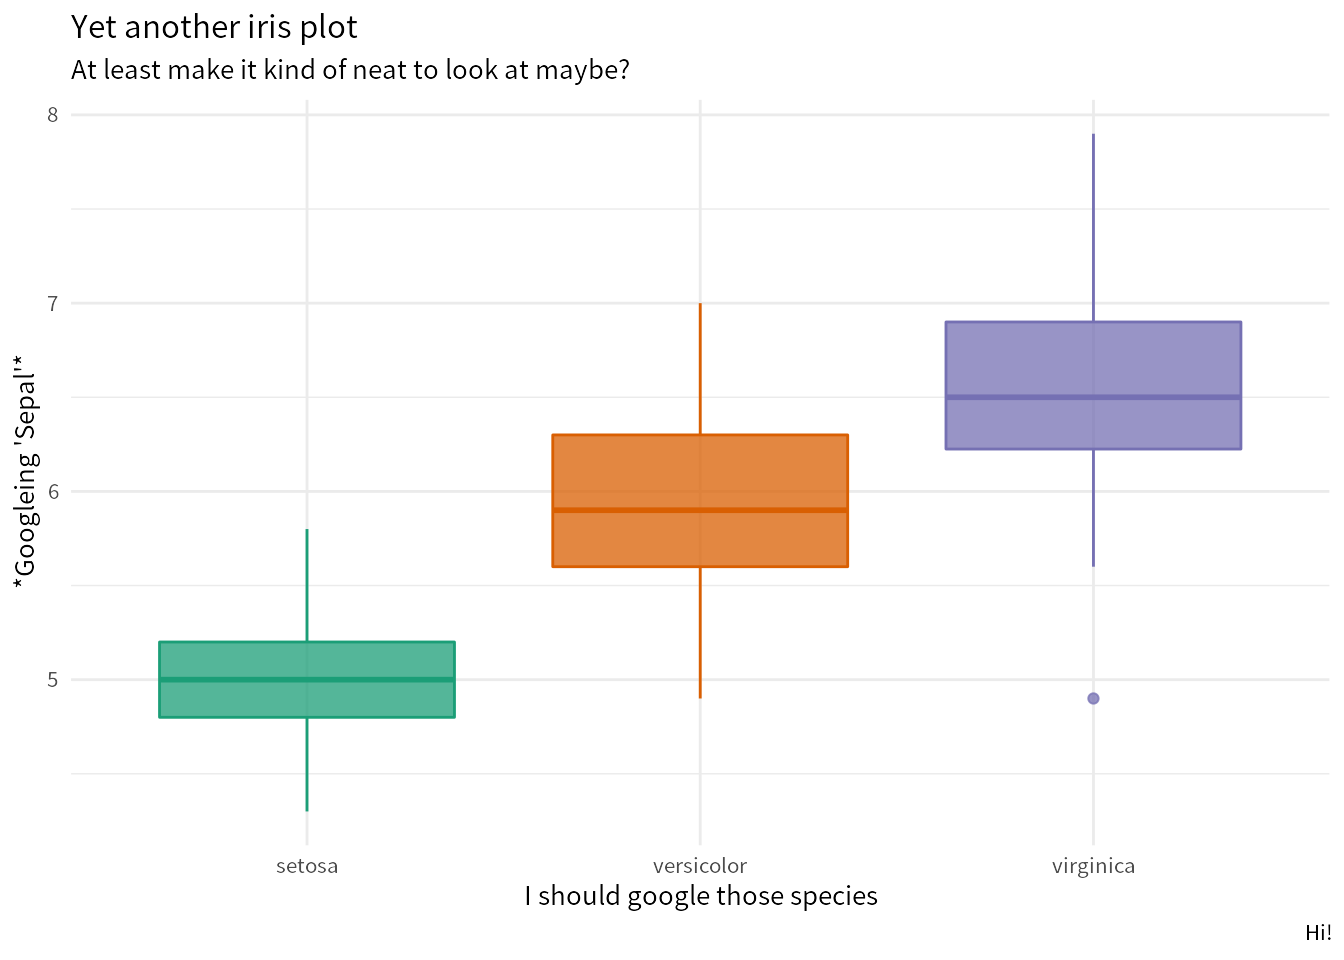
\includegraphics{bookdown-debugging_files/figure-latex/plotting-1-2.pdf}
\caption{\label{fig:plotting-1-2}A plot.}
\end{figure}

\begin{Shaded}
\begin{Highlighting}[]
\NormalTok{p }\OperatorTok{+}\StringTok{ }\KeywordTok{theme_minimal}\NormalTok{(}\DataTypeTok{base_family =} \StringTok{"Roboto Condensed"}\NormalTok{) }\OperatorTok{+}
\StringTok{   }\KeywordTok{labs}\NormalTok{(}\DataTypeTok{subtitle =} \StringTok{"Using Roboto Condense"}\NormalTok{)}
\end{Highlighting}
\end{Shaded}

\begin{figure}
\centering
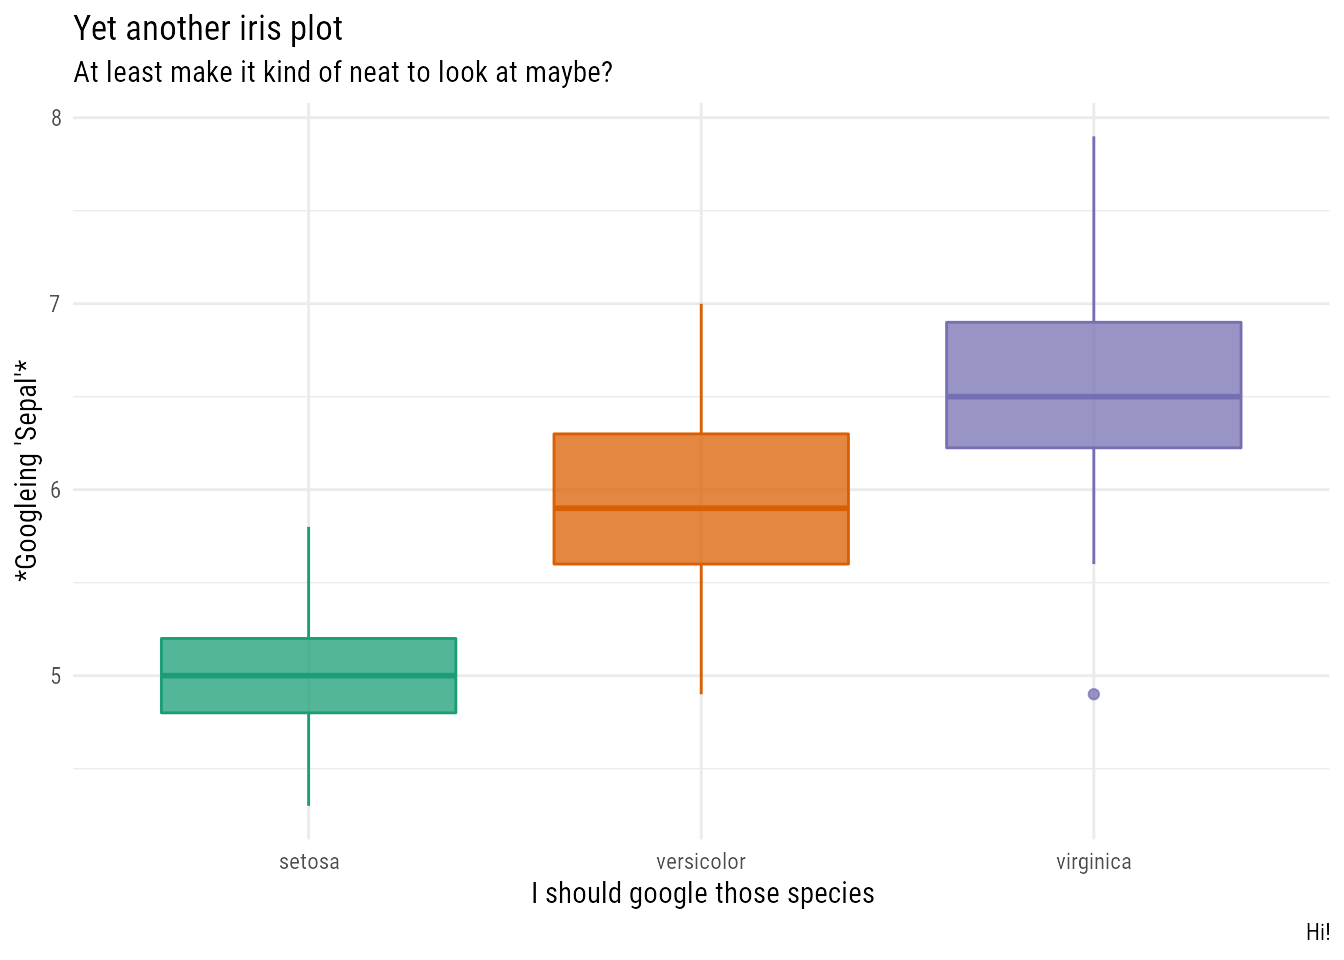
\includegraphics{bookdown-debugging_files/figure-latex/plotting-1-3.pdf}
\caption{\label{fig:plotting-1-3}A plot.}
\end{figure}

\begin{Shaded}
\begin{Highlighting}[]
\KeywordTok{library}\NormalTok{(hrbrthemes)}
\end{Highlighting}
\end{Shaded}

\begin{verbatim}
## NOTE: Either Arial Narrow or Roboto Condensed fonts are required to use these themes.
\end{verbatim}

\begin{verbatim}
##       Please use hrbrthemes::import_roboto_condensed() to install Roboto Condensed and
\end{verbatim}

\begin{verbatim}
##       if Arial Narrow is not on your system, please see https://bit.ly/arialnarrow
\end{verbatim}

\begin{Shaded}
\begin{Highlighting}[]
\NormalTok{p }\OperatorTok{+}\StringTok{ }\KeywordTok{theme_ipsum_rc}\NormalTok{() }\OperatorTok{+}
\StringTok{   }\KeywordTok{labs}\NormalTok{(}\DataTypeTok{subtitle =} \StringTok{"Using hrbrthemes::theme_ipsum_rc()"}\NormalTok{)}
\end{Highlighting}
\end{Shaded}

\begin{figure}
\centering
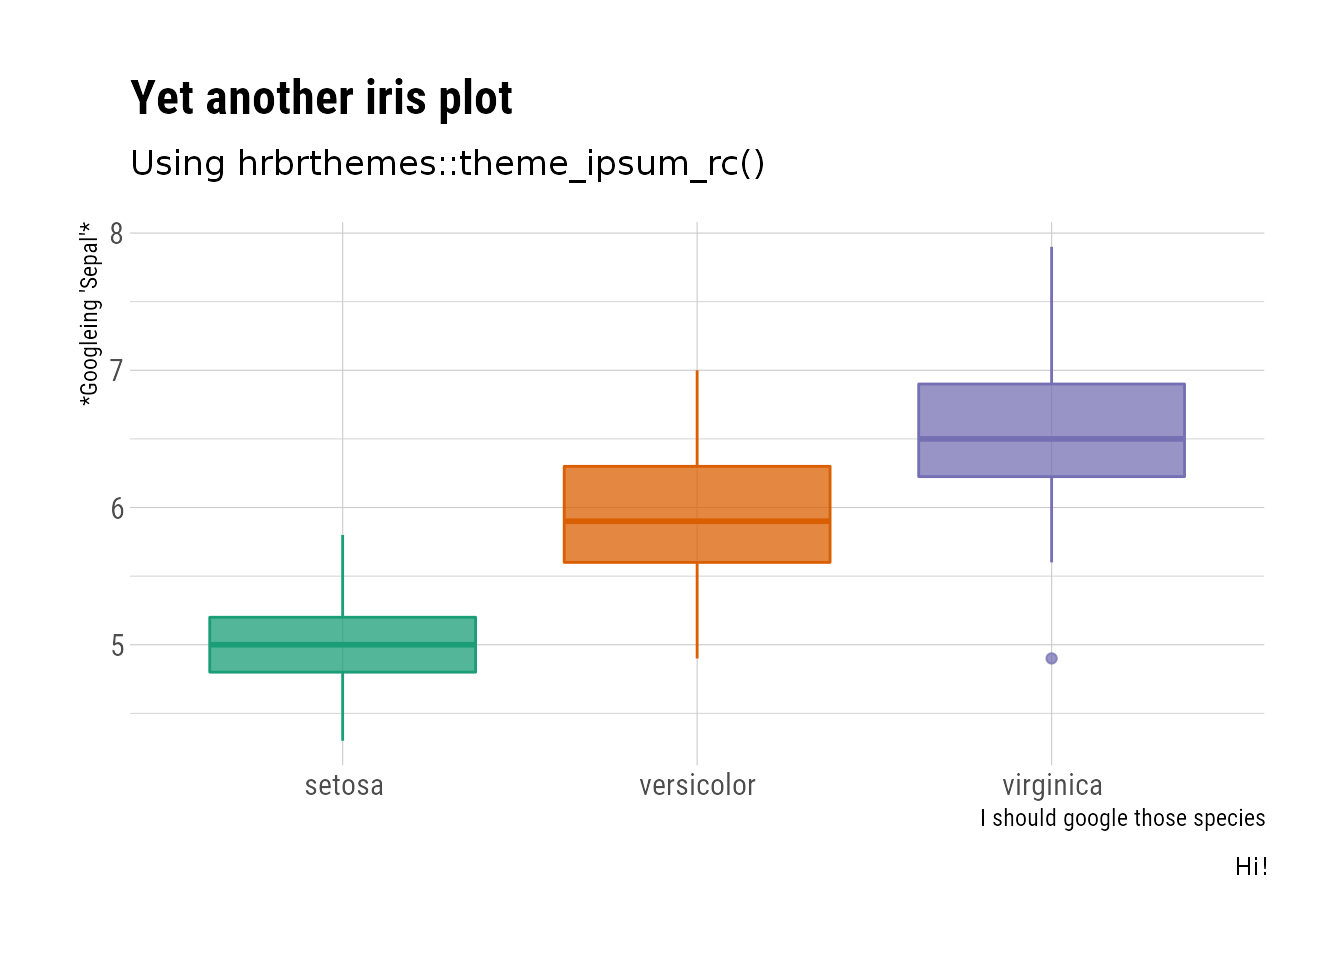
\includegraphics{bookdown-debugging_files/figure-latex/plotting-1-4.pdf}
\caption{\label{fig:plotting-1-4}A plot.}
\end{figure}

\hypertarget{math}{%
\subsection{Math}\label{math}}

Using one dollar sign: \(\beta = (X^T X)^{-1} X^T Y\)

Display style with two dollar signs:

\[\beta = (X^T X)^{-1} X^T Y\]

\hypertarget{using-environments}{%
\subsubsection{Using environments}\label{using-environments}}

Below should be a set of equations using an \texttt{align} environment. If not, I still don't understand MathJax.

\begin{align}
\mathbb{E}(\widehat{\boldsymbol{\beta}}) 
&= \mathbb{E}\left( \left(\boldsymbol{X}^T \boldsymbol{X}\right)^{-1} \boldsymbol{X}^T \boldsymbol{Y} \right) \\
&= \mathbb{E}\left( \left(\boldsymbol{X}^T \boldsymbol{X}\right)^{-1} \boldsymbol{X}^T \left(\boldsymbol{X} \boldsymbol{\beta}+ \varepsilon \right) \right) \\
&= \mathbb{E}\left( 
   \left(\boldsymbol{X}^T \boldsymbol{X}\right)^{-1} \boldsymbol{X}^T \boldsymbol{X} \boldsymbol{\beta} 
 + \left(\boldsymbol{X}^T \boldsymbol{X}\right)^{-1} \boldsymbol{X}^T \boldsymbol{\varepsilon}
   \right) \\
&= \underbrace{\left(\boldsymbol{X}^T \boldsymbol{X}\right)^{-1} \boldsymbol{X}^T \boldsymbol{X}}_{=\ \boldsymbol{I}} \boldsymbol{\beta} 
 + \underbrace{\left(\boldsymbol{X}^T \boldsymbol{X}\right)^{-1} \boldsymbol{X}^T \mathbb{E}(\boldsymbol{\varepsilon})}_{=\ 0}
 & \Bigg\vert\ \mathbb{E}(\boldsymbol{\varepsilon}) = 0\\
&= \boldsymbol{\beta} & \Box
\end{align}

\texttt{equation} from bookdown book:

\begin{equation} 
  f\left(k\right) = \binom{n}{k} p^k\left(1-p\right)^{n-k}
  \label{eq:binom}
\end{equation}

\hypertarget{applications}{%
\section{Applications}\label{applications}}

Some \emph{significant} applications are demonstrated in this chapter.

\hypertarget{example-one}{%
\subsection{Example one}\label{example-one}}

\hypertarget{example-two}{%
\subsection{Example two}\label{example-two}}

\hypertarget{session-info}{%
\section{Session info}\label{session-info}}

\begin{Shaded}
\begin{Highlighting}[]
\NormalTok{sessioninfo}\OperatorTok{::}\KeywordTok{session_info}\NormalTok{()}
\end{Highlighting}
\end{Shaded}

\begin{verbatim}
## - Session info ---------------------------------------------------------------
##  setting  value                       
##  version  R version 4.0.0 (2020-04-24)
##  os       Ubuntu 16.04.6 LTS          
##  system   x86_64, linux-gnu           
##  ui       X11                         
##  language en_US.UTF-8                 
##  collate  en_US.UTF-8                 
##  ctype    en_US.UTF-8                 
##  tz       UTC                         
##  date     2020-05-07                  
## 
## - Packages -------------------------------------------------------------------
##  ! package      * version date       lib source                      
##  P assertthat     0.2.1   2019-03-21 [?] CRAN (R 4.0.0)              
##  P bookdown       0.18    2020-03-05 [?] CRAN (R 4.0.0)              
##  P cli            2.0.2   2020-02-28 [?] CRAN (R 4.0.0)              
##  P colorspace     1.4-1   2019-03-18 [?] CRAN (R 4.0.0)              
##  P crayon         1.3.4   2017-09-16 [?] CRAN (R 4.0.0)              
##  P digest         0.6.25  2020-02-23 [?] CRAN (R 4.0.0)              
##  P ellipsis       0.3.0   2019-09-20 [?] CRAN (R 4.0.0)              
##  P evaluate       0.14    2019-05-28 [?] CRAN (R 4.0.0)              
##  P extrafont    * 0.17    2014-12-08 [?] CRAN (R 4.0.0)              
##  P extrafontdb    1.0     2012-06-11 [?] CRAN (R 4.0.0)              
##  P fansi          0.4.1   2020-01-08 [?] CRAN (R 4.0.0)              
##  P farver         2.0.3   2020-01-16 [?] CRAN (R 4.0.0)              
##  P gdtools        0.2.2   2020-04-03 [?] CRAN (R 4.0.0)              
##  P ggplot2      * 3.3.0   2020-03-05 [?] CRAN (R 4.0.0)              
##    glue           1.4.0   2020-04-03 [1] CRAN (R 4.0.0)              
##  P gtable         0.3.0   2019-03-25 [?] CRAN (R 4.0.0)              
##  P highr          0.8     2019-03-20 [?] CRAN (R 4.0.0)              
##  P hrbrthemes   * 0.8.0   2020-03-06 [?] CRAN (R 4.0.0)              
##  P htmltools      0.4.0   2019-10-04 [?] CRAN (R 4.0.0)              
##  P knitr          1.28.7  2020-05-07 [?] Github (yihui/knitr@6907b42)
##  P labeling       0.3     2014-08-23 [?] CRAN (R 4.0.0)              
##  P lifecycle      0.2.0   2020-03-06 [?] CRAN (R 4.0.0)              
##  P magrittr       1.5     2014-11-22 [?] CRAN (R 4.0.0)              
##  P munsell        0.5.0   2018-06-12 [?] CRAN (R 4.0.0)              
##  P pillar         1.4.4   2020-05-05 [?] CRAN (R 4.0.0)              
##  P pkgconfig      2.0.3   2019-09-22 [?] CRAN (R 4.0.0)              
##  P R6             2.4.1   2019-11-12 [?] CRAN (R 4.0.0)              
##  P ragg         * 0.1.5   2020-03-04 [?] CRAN (R 4.0.0)              
##  P RColorBrewer   1.1-2   2014-12-07 [?] CRAN (R 4.0.0)              
##    Rcpp           1.0.4.6 2020-04-09 [1] CRAN (R 4.0.0)              
##    renv           0.10.0  2020-05-06 [1] CRAN (R 4.0.0)              
##    rlang          0.4.6   2020-05-02 [1] CRAN (R 4.0.0)              
##  P rmarkdown      2.1     2020-01-20 [?] CRAN (R 4.0.0)              
##  P rstudioapi     0.11    2020-02-07 [?] CRAN (R 4.0.0)              
##  P Rttf2pt1       1.3.8   2020-01-10 [?] CRAN (R 4.0.0)              
##  P scales         1.1.0   2019-11-18 [?] CRAN (R 4.0.0)              
##  P sessioninfo    1.1.1   2018-11-05 [?] CRAN (R 4.0.0)              
##  P stringi        1.4.6   2020-02-17 [?] CRAN (R 4.0.0)              
##  P stringr        1.4.0   2019-02-10 [?] CRAN (R 4.0.0)              
##  P systemfonts    0.2.1   2020-04-29 [?] CRAN (R 4.0.0)              
##  P tibble         3.0.1   2020-04-20 [?] CRAN (R 4.0.0)              
##  P vctrs          0.2.4   2020-03-10 [?] CRAN (R 4.0.0)              
##  P withr          2.2.0   2020-04-20 [?] CRAN (R 4.0.0)              
##    xfun           0.13    2020-04-13 [1] CRAN (R 4.0.0)              
##  P yaml           2.2.1   2020-02-01 [?] CRAN (R 4.0.0)              
## 
## [1] /home/travis/build/jemus42/bookdown-debugging/renv/library/R-4.0/x86_64-pc-linux-gnu
## [2] /tmp/Rtmpw4Gsp4/renv-system-library
## 
##  P -- Loaded and on-disk path mismatch.
\end{verbatim}

\bibliography{book.bib,packages.bib}

\end{document}
